\documentclass[a4paper,norsk,12pt]{report}

\usepackage[norsk]{babel}
\usepackage{enumitem}
\usepackage{color}
\usepackage{amsmath}
\usepackage{wrapfig}
\usepackage{graphicx}
\usepackage[utf8]{inputenc}
\usepackage{multirow,tabularx}
\usepackage{setspace}
\usepackage{hyperref}
\onehalfspacing
\newcolumntype{Y}{>{\centering\arraybackslash}X}
\renewcommand{\arraystretch}{2}
\renewcommand*{\chaptername}{Del}

\pagestyle{empty}

\begin{document}
\chapter{Bakgrunn og teorigrunnlag}
\chapter{}
\section{Datainnsamling}
For å undersøke om det er forskjell i læringseffekt når undervisningen organiseres rundt forelesninger eller når den organiseres rundt oppgaveregning med tilhørende diskusjon har jeg testet begge studentgruppene før og etter nytt fagstoff ble undervist. Testen er av en slik art at man selv uten fagkunnskaper vil være i stand til å gjøre seg opp en mening om hva som er riktig svar, men testen er designet for å avsløre vanlige misoppfatninger. Dermed vil man forvente at en student uten aktuelle fagkunnskaper vil få en dårlig uttelling.

I forbindelse med testing av forkunnskaper har jeg også bedt studentene om å oppgi litt informasjon om bakgrunnen deres. Spesifikt har jeg spurt om:
\begin{itemize}
\item
	Hvilke matematikk-kurs de har tatt på videregående skole
\item
	Hvilke fysikk-kurs de har tatt på videregående skole
\item
	Om de har vært gjennom realfagskurs eller forkurs før de startet på høyskolestudiene
\item
	Hvilken karakter de fikk i MAT100/MA2-100/MAT108 (Matematikk-kurs ved HVL som gir nødvendig matematisk grunnlag for å studere fysikk).
\end{itemize}

\subsection{Beskrivelse av testen}
Testen jeg bruker til å teste fysikk-kunnskapene til studentene heter Force Concept Inventory \cite{1992FCI}. Testen er utviklet ved Arizona State University og oversatt til norsk ved Skolelaboratoriet, Universitetet i Oslo. Testen består av 30 flervalgsoppgaver om krefter (Newtonsk mekanikk). Alle spørsmål er av ren kvalitativ art og tar dermed sikte på å teste fysikk-forståelse uavhengig av matematiske kunnskaper. 

Force Concept Inventory oppfyller PhysPort\footnote{PhysPort (\url{https://www.physport.org/} er en ressursside for fysikk-undervisere med fokus på forsknings-basert undervisningspraksis. PhysPort er utviklet av American Association for Physics Teachers i samarbeid med Kansas State University.)} sine kriterier til "gull-standard", hvilket innebærer at \cite{2014arXiv1404.6500M}:
\begin{itemize}
\item
Spørsmålene er basert på forskning på hvordan studenter tenker.
\item
Testen er validert ved hjelp av student-intervjuer.
\item
Testen er validert av fag-eksperter.
\item
Testen er validert med tilfredsstillende statistisk analyse.
\item
Testen er brukt ved flere institusjoner.
\item
Testen er brukt i forskning gjort av andre enn utviklerne av testen.
\item
Testen er brukt i minst en fagfelle-vurdert publikasjon.
\end{itemize}

\subsection{Beskrivelse av datainnsamlingen}
Den samme testen ble gitt til studentene to ganger---i første undervisningsuke og i femte undervisningsuke, uken etter gjennomgang av den delen av pensum som er relevant for testen var ferdig. Studentene visste at de skulle testes på nytt, men de visste ikke at de to testene var identisk. De hadde heller ikke tilgang til testspørsmålene i tiden mellom de to testene. 

Testingen ble gjennomført elektronisk ved hjelp av \emph{SMART response 2} som er innebygget i programmet \emph{SMART Notebook} \cite{smart} som er installert i alle undervisningsrom på HVL/Kronstad. Når dette programmet brukes logger studentene seg inn på en nettside og får opp spørsmålene og leverer svar på egen datamaskin/telefon. De kan under hele testen gå frem og tilbake mellom de ulike spørsmålene, men de har kun tilgang til spørsmålene i den tiden datainnsamlingen er aktivert. Studentene svarte individuelt og ble bedt om å ikke diskutere spørsmålene underveis, men dette ble ikke håndhevet strengt. 

For at studentene skulle kunne svare anonymt samtidig som det var mulig å koble svar fra samme student avgitt på testen før undervisningsperioden og testen etter eksamensperioden ble studentene bedt om å logge seg inn i med et selvvalgt kallenavn. Det ble understreket før den første testen at de måtte bruke samme kallenavn også på den andre testen. Dette ble igjen understreket før den andre testen, og de fikk da også se listen over kallenavn som var brukt ved første test for å lettere kunne huske hva de selv hadde brukt. Det var imidlertid en del som likevel ikke logget seg inn med likt kallenavn på de to testene, og dermed måtte en del data forkastes. Det fantes ikke noen kontrollmekanisme som sikret at det i de tilfellene samme kallenavn var brukt på begge testene, faktisk var samme student begge ganger.

Både ved testen før undervisning og etter undervisning ble studentene bedt om å svare på om de godkjente at svarene dere blir brukt til læringsanalyse. Svarene fra studenter som ikke godkjente dette er ikke brukt videre i analysen.

\subsection{Beskrivelse av datasettene}
Data-innsamlingen som er beskrevet ovenfor gir opphav til tre datasett:
\begin{itemize}
\item
	bakgrunnsinformasjon (bgData)
\item
	testresultater fra test før undervisning (preData)
\item
	testresultater fra test etter undervisning (postData)
\end{itemize}
Siden læringsanalysen krever kobling av de ulike datasettene har jeg gjort følgende utvalg fra disse datasettene for bruk i analyse
\begin{itemize}
\item
	bakgrunnsinformasjon og testresultater for de studentene der kobling av disse er vellykket (matchPreData)
\item
	testresultater fra før-test og etter-test for de studentene der kobling av disse er vellykket (matchPostData)
\end{itemize}
I koblingen mellom preData og postData krever jeg ikke en samtidig kobling med bgData. Dette ville vært nødvendig hvis jeg dataanalysen skulle undersøkt om skole/studie-bakgrunn påvirker læringen, men datasettet jeg har samlet inn er for lite til å kunne gjøre en meningsfull analyse av dette.

Tabell \ref{tab:predata}-\ref{tab:postdata} oppsummerer hvor mange studenter fra hvert av kursene som er med i hvert datasett.
\begin{table}[tp]
\begin{tabularx}{\textwidth}{|*{3}{Y|}}
\hline
& DAT106 & BYG103/BYG141 \\
\hline
bgData & 26 & 113 \\
\hline
preData & 27 & 115 \\
\hline
matchPreData & 24  & 89  \\
\hline
\end{tabularx}
\caption{Antall studenter per kurs og per datasett i data samlet inn før undervisning. bgData er data om studentens skole/studie-bakgrunn. preData er resultater fra testen før undervisning. matchPreData er de studentene der det er en vellykket kobling mellom bgData og preData.}
\label{tab:predata}
\end{table}

\begin{table}[tp]
\begin{tabularx}{\textwidth}{|*{3}{Y|}}
\hline
& DAT106 & BYG103/BYG141 \\
\hline
postData & & \\
\hline
matchPostData & &  \\
\hline
\end{tabularx}
\caption{Antall studenter per kurs og per datasett i data samlet inn etter undervisning. postData er resultater fra testen etter undervisning. matchPostData er de studentene der det er en vellykket kobling mellom preData og postData.}
\label{tab:postdata}
\end{table}

\section{Undervisningsform}
\subsection{BYG103/BYG141}
Kurset BYG103/BYG141 er et felleskurs for bygg- og anleggsingeniør-studenter i Bergen og Førde (derav to ulike kurskoder). Studentene tar dette kurset i andre semester. I første semester har studentene tatt matematikk-kurset MAT100 (Bergen) eller MA2-100 (Førde) som inneholder blant annet vektorregning, derivasjon og integrasjon som er nødvendige forutsetninger for lærestoffet i BYG103/BYG141. Parallelt med fysikk-forelesningen i BYG103/BYG141 foreleses det også statikk som gir studentene ytterligere trening i vektorregning.

Undervisningen er lokalisert i Auditorium 2 (187 plasser) i Bergen med videokonferanse til Auditorium Nordfjord i Førde. Typisk antall fremmøtte til undervisningen er ca 100 i Bergen og mindre enn 10 i Førde. Fysikk-delen av kurset har tre undervisningstimer i uken; tirsdager fra 14:15-17:00. De to første undervisningstimene bruker jeg til forelesning. I hovedsak bruker jeg en tradisjonell forelesningform, men for å skape litt variasjon bryter jeg innimellom av forlesningene med korte øvelser for studentene. Det er i hovedsak to typer avbrudd jeg bruker:
\begin{itemize}
\item
Studentene får en enkel regneoppgave som konkretiserer teori som nettopp er gjennomgått. Studentene får her først en del minutter for å forsøke å løse oppgaven selv---gjerne i samarbeid med den/de som sitter ved siden av---før jeg gjennomgår oppgaven i plenum.
\item
Kvalitative flervalgsspørsmål besvart via telefon/datamaskin. Spørsmålene er laget for å undersøke om studentene har forstått teorien vi nettopp har gjennomgått. Statistikk over fordelingen av svar er straks tilgjengelig, slik at jeg kan bruke ekstra tid på å diskutere de temaene der det viser seg at mange ikke har god nok forståelse ennå.
\end{itemize}
Den siste undervisningstimen brukes til å gjennomgå regneoppgaver. På grunn av stort antall studenter og fordeling på to campuser ser jeg det ikke som en aktuell mulighet å la studentene sitte å regne selv mens jeg går rundt å hjelper. I stedet får de oppgavesettet omtrent en uke på forhånd slik at de på egenhånd kan forsøke på oppgavene før jeg viser i plenum hvordan de kan løses. I tillegg lager jeg skriftlig løsningsforslag som jeg gjør tilgjengelig etter at regnetimen er ferdig.

\subsection{DAT106}
Kurset DAT106 er et kurs for dataingeniørstudenter. Kurset består av 7 studiepoeng fysikk og 3 studiepoeng kjemi. Studentene tar kurset i fjerde semester. Tidligere i studiet har studentene tatt matematikk-kursene MAT101, MAT102 og MAT108. MAT108 som studentene tok i andre semester inneholder vektorregning, derivasjon- og integrasjon.

Undervisningen er lokalisert i ulike klasserom på Kronstad. Typisk romstørrelse er til 40 personer, og typisk antall fremmøte er 20. Det er to dobbeltimer hver uke. Hver dobbeltime starter med en kort oppsummeringsforelesning av det lærestoffet som vi skal arbeide med i timen---og som studentene har blitt oppfordret til å lese på forhånd. Resten av tiden brukes til oppgaveregning. Jeg oppfordret studentene til å jobbe i grupper. I denne delen av av timen har jeg i hovedsak gått rundt å hjulpet studentene---fortrinnsvis ved å dytte diskusjonen deres i riktig retning mer enn å direkte fortelle dem hvordan problemet skal løses. Erfaringen min var at i noen studentgrupper fungerte dette svært bra: Studentene diskuterte ivrig sammen og fra det jeg kunne høre fikk de belyst problemet fra ulike sider. Når de følte at de enten var i en blindgate eller ikke ble enig om hvilken løsning som var riktig tok de meg med inn i diskusjonen. Andre studenter var langt mindre ivrige i diskusjonen, og spørsmålene deres var mer operasjonelle.

Utvalge av oppgaver til regneøvingen er det samme som for BYG103/BYG141, og også DAT106-studentene fikk tilgang til skriftlig løsningsforslag etter hver undervisningsuke. 


\section{Resultater}
Figur \ref{fig:testScore} sammenligner fordelingen av testresultatene før (venstre) og etter (høyre) undervisningen for de to studentgruppene. Resultatene fra testen før undervisning inkluderer alle studentene i datasettet preData (115+27 studenter), mens resultatene fra testen etter undervisning inkluderer studentene fra datasettet matchPreData (89+24 studenter). Når en stor andel av studentene som deltok i testen første gang ikke deltok i testen andre gang kan resultater tolket ut fra disse histogrammene skyldes en utvalgsbias. Figur \ref{fig:testScoreMatch} viser derfor de samme histogrammene, men kun med studenter fra datasettet matchPreData inkludert. Histogrammet for resultater etter test er identisk i figur \ref{fig:testScore} og \ref{fig:testScoreMatch}, men er gjentatt for å gjøre sammenligningen enklere.
\begin{figure}[p]
	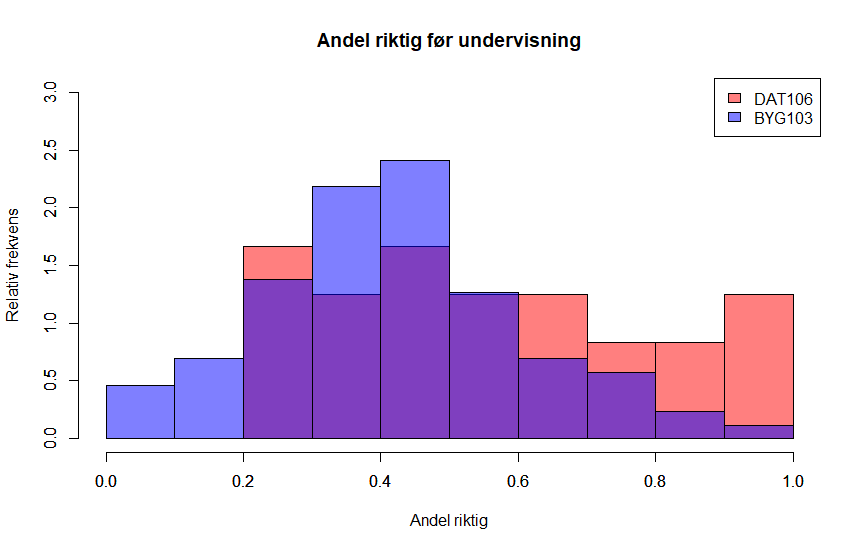
\includegraphics[width=.48\textwidth]{./preScoreAll}
	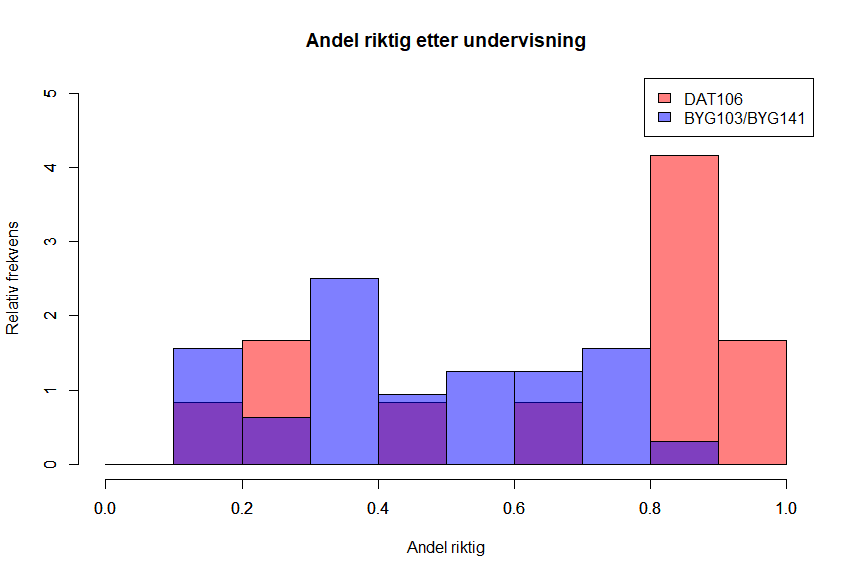
\includegraphics[width=.48\textwidth]{./postScore}
	\caption{Sammenligning av testresultater for studenter fra kursene DAT106 og  BYG103/BYG141 før (venstre) og etter (høyre) undervisningsperioden. Histogrammet med før-resultater 
baserer seg på flere studenter enn histogrammet for etter-resultater siden færre studenter valgte å delta på testen andre gang.}
	\label{fig:testScore}
\end{figure}

\begin{figure}[p]
	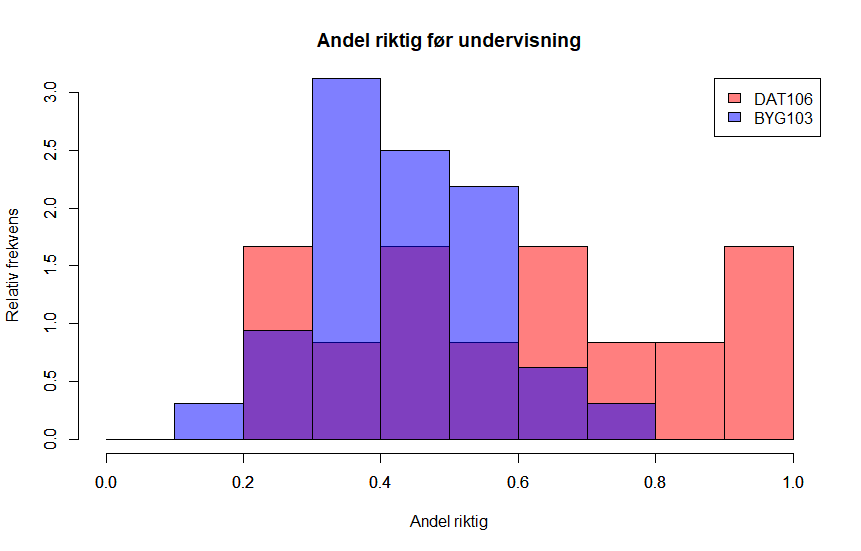
\includegraphics[width=.48\textwidth]{./preScore}
	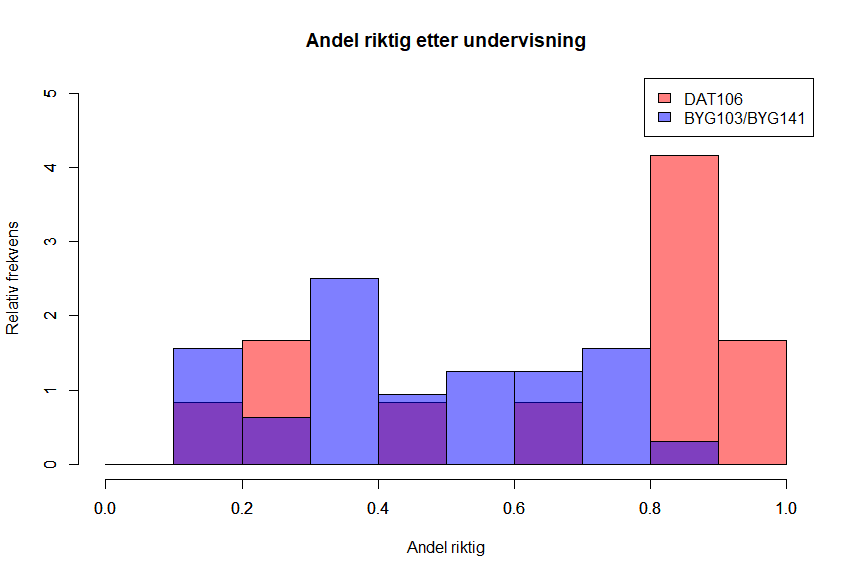
\includegraphics[width=.48\textwidth]{./postScore}
	\caption{Sammenligning av testresultater for studenter fra kursene DAT106 og  BYG103/BYG141 før (venstre) og etter (høyre) undervisningsperioden. Kun studenter som deltok på både før- og etter-testene er inkludert i histogrammene.}
	\label{fig:testScoreMatch}
\end{figure}

For de studentene som deltok på både før- og etter-testen er utviklingen i resultat vist i figur \ref{fig:forbedring}. Histogrammet til venstre viser absolutt forbedring, altså $S_\text{etter}-S_\text{før}$ der $\eta_\text{abs} = S_\text{før}$ og $S_\text{etter}$ er andel riktig i testen henholdsvis før og etter undervisningsperioden. Histogrammet til høyre viser den relative forbedringen definert som
\begin{displaymath}
	\eta_\text{rel} = \frac{S_\text{etter}-S_\text{før}}{1 - S_\text{før}}.
\end{displaymath}
Den relative forbedringen kan tolkes som hvor stor andel av spørsmålene som var feil besvart første gang som ble riktig besvart andre gang. Merk at denne variablen har en svakhet for studenter som hadde et svært godt resultat ved første test: Hvis en av disse studenten gjør kun \'en feil mer i andre forsøk enn i første forsøk får den relative forbedringen en stor negativ verdi.
\begin{figure}[p]
	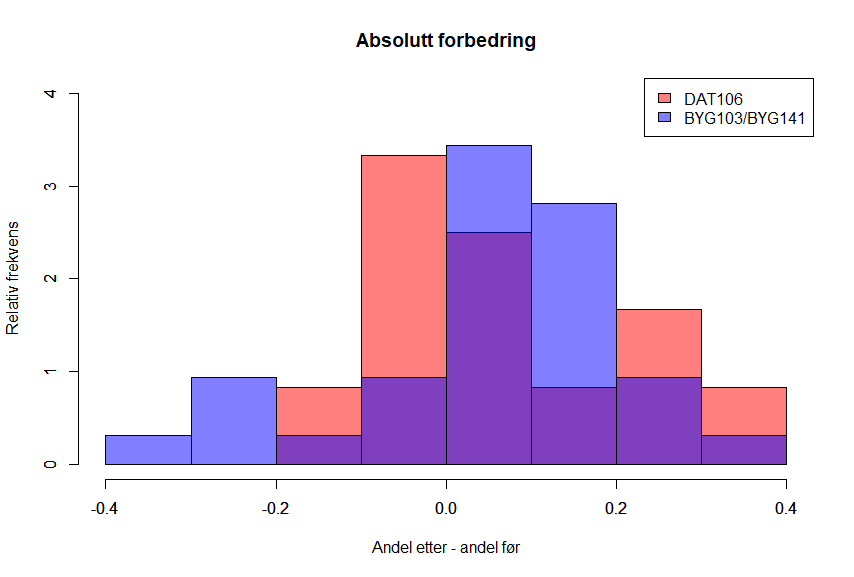
\includegraphics[width=.48\textwidth]{./absForbedring}
	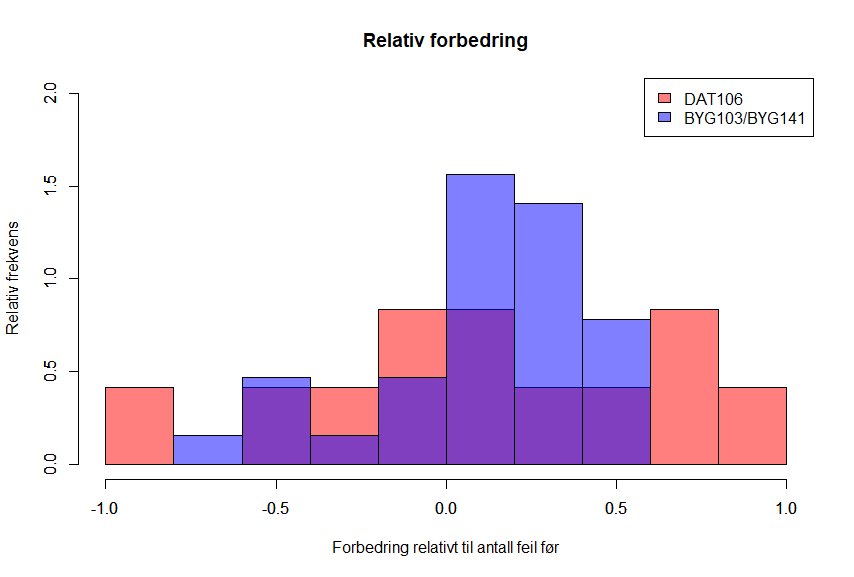
\includegraphics[width=.48\textwidth]{./relForbedring}
	\caption{}
	\label{fig:forbedring}
\end{figure}
For å kunne undersøke hvorvidt studentens forkunnskaper påvirker hvor godt resultat de ulike gir er det i figur \ref{fig:scatter} vist resultat av før-testen plottet mot absolutt forbedring (venstre) og relativ forbedring (høyre). 
\begin{figure}[p]
	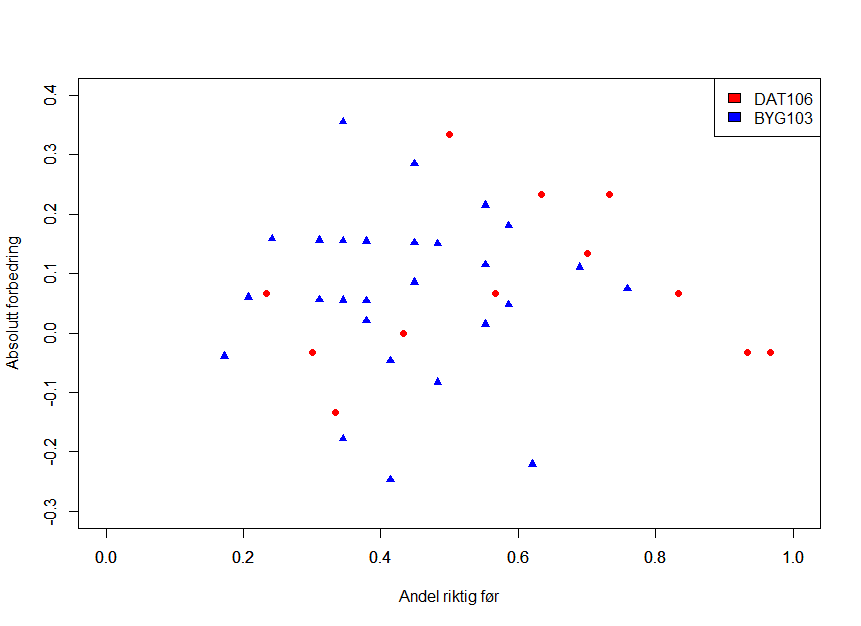
\includegraphics[width=.48\textwidth]{./absoluttForbedringScatter}
	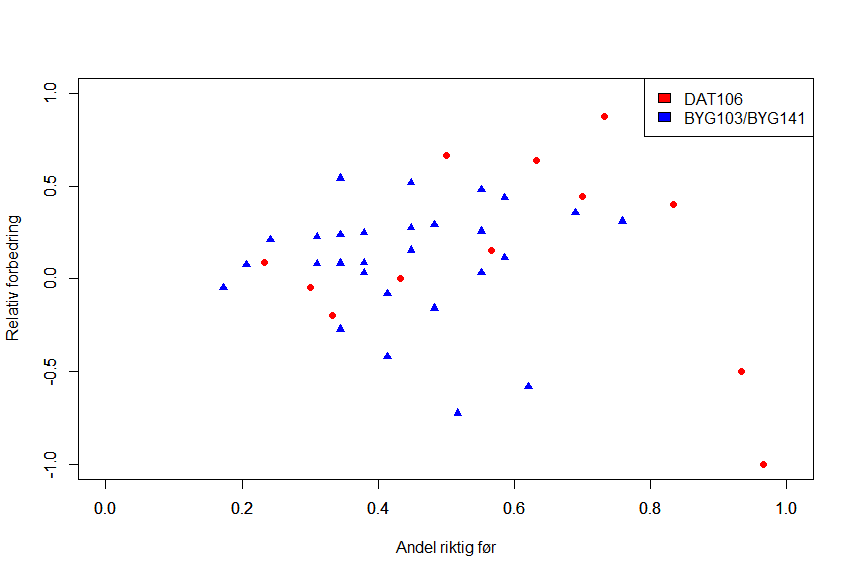
\includegraphics[width=.48\textwidth]{./relativForbedringScatter}
	\caption{}
	\label{fig:scatter}
\end{figure}

\subsection{Betydningen av studiebakgrunn}
Datasettet som er samlet inn er ikke stort nok til å gjøre en studie av i hvilken grad ulike aspekter ved studentenes bakgrunn før de startet på DAT106 eller BYG103/BYG141 påvirker læringsutbyttet. Derfor begrenser dette avsnittet seg til å presentere resultater for sammenhengen mellom studentenes bakgrunn og resultatene de oppnådde på testen før undrevisningsperioden. Dette har imidlertid egen-interesse utover hovedmålsetningen med prosjektet mitt, og er derfor verdt å undersøke. Datasettet som er brukt for denne delen av studien er matchPreData. I noen tilfeller er imidlertid ikke alle studentene i dette datasettet inkludert, da matchingen ikke krever at de har svart på alle spørsmålene om studiebakgrunn.

Figur \ref{fig:fysmat} viser andel riktig på før-testen for studenter med/uten Fysikk 2 (venstre) og Matematikk R2 (høyre) fra videregående skole. Dette er kurs som ikke utgjør en del av opptakskravet for ingeniørstudiene, men som gir studentene en større fordypning i fysikk og matematikk enn minimumskravet. Det er dermed interessant å undresøke om dette påvirker testresultatene.
\begin{figure}[p]
	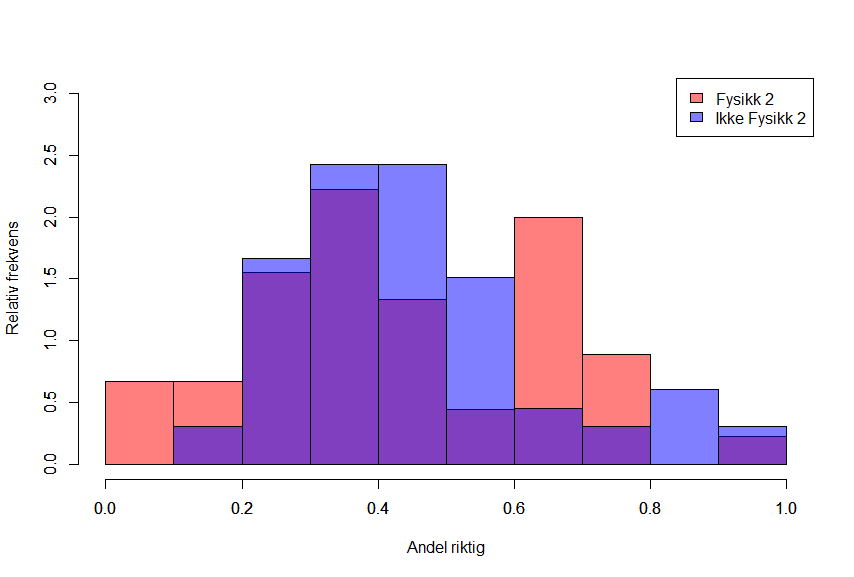
\includegraphics[width=.48\textwidth]{./fys2}
%	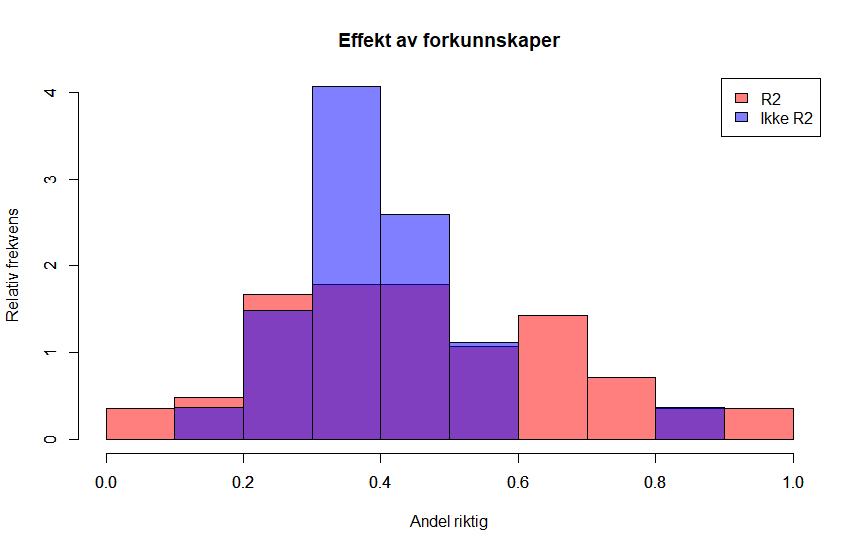
\includegraphics[width=.48\textwidth]{./r2}
	\caption{}
	\label{fig:fysmat}
\end{figure}
Elever som ikke har tilstrekkelig fordypning i matematikk og fysikk fra videregående kan oppnå påkrevd kompetanse for å starte på ingeniørstudier gjennom å ta enten forkurs eller realfagskurs {\color{red}[Fyll inn detaljer. Snakk med Kristine]}. Figur \ref{fig:forkurs} viser andel riktig på før-testen for studenter som har bakrunn fra enten realfagskurs (venstre) eller forkurs (høyre). I begge tilfeller er resultatene sammenlignet med studenter som er tatt opp på studiet med tilstrekkelig fordypning i matematikk og fysikk fra videregående skole.
\begin{figure}[p]
	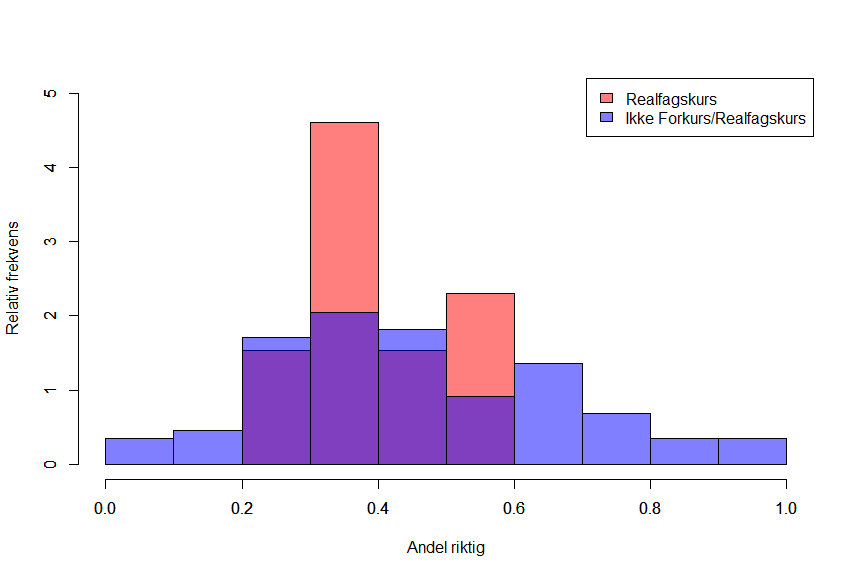
\includegraphics[width=.48\textwidth]{./real}
%	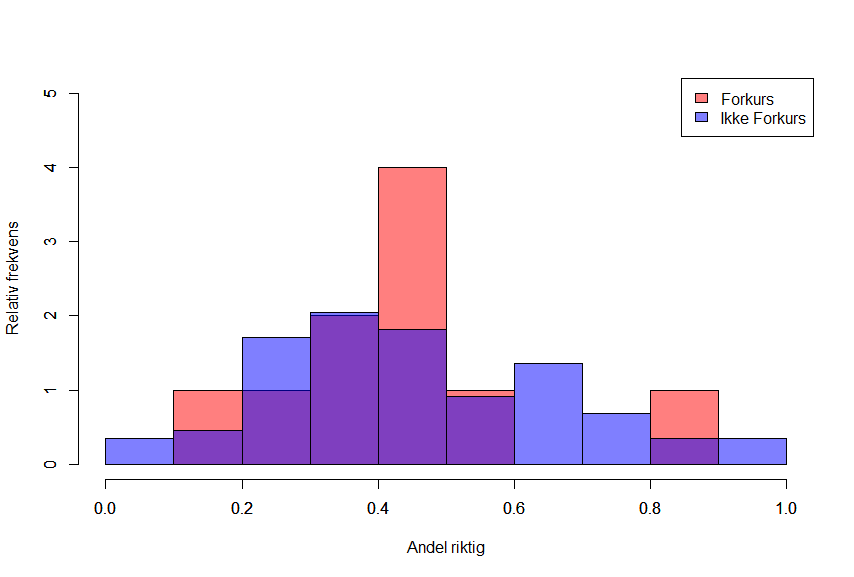
\includegraphics[width=.48\textwidth]{./forkurs}
	\caption{ Sammenligning av resultater for studenter som har tilstrekkelig matematikk- og fysikk-bakgrunn fra videregående skole (blå) med studenter som har tatt realfagskurs (venstre) eller forkurs (høyre) for å oppfylle opptakskravet til ingeniørstudier (rød).}
	\label{fig:fysmat}
\end{figure}




\chapter{Diskusjon av resultatene}

\section{Sammenligning av tradisjonell forelesning og omvendt klasserom}
Det primære målet for denne studien var å undersøke om ''omvent klasserom''---som en representant for studentaktive læringsformer---gir bedre læringsutbytte for studentene enn ''tradisjonell forelesning''. En sammenligning av resultatene fra testen før undervisningsperioden og etter undervisningsperioden, vist i figurene \ref{fig:testScore}-\ref{fig:testScoreMatch}, viser at begge studentgruppene har bedret resultatet sitt---hvilket selvfølgelig er målet med undervisningen uansett hvordan den er organisert. Det tydeligste bildet får vi fra figur \ref{fig:testScoreMatch} der det er nøyaktig den samme studentpopulasjonen som er brukt i histogrammet for resultater før og etter testen. Ved å sammeligne på denne måten tar vi vekk utvalgsbiasen som kan komme dersom det er en korrelasjon mellom resultatet på første test og hvorvidt en student velger å delta på andre test eller ikke. Sammenligning av første histogram i henholdsvis figur \ref{fig:testScore} og \ref{fig:testScoreMatch} viser at det til en viss grad er en slik utvalgsbias til stede: Spesielt i BYG103/BYG141 ser vi at en større andel av studentene med de sterkeste og de svakeste resultatene på første test valgte å ikke ta andre test. I DAT106 er utvalgsbiasen mindre, men også her ser vi en tendens til at studenter fra svakeste halvpart på første test i større grad valgte å ikke ta andre test. 

For å evaluere endringen mellom første og andre test er det nyttig å studere histogram som viser forbedringen som vist i figur \ref{fig:forbedring}. Ut fra histogrammene kan vi se at gruppen med omvent klasserom (DAT106) har i gjennomsnitt noe bedre fremgang enn gruppen med forelesninger (BYG103/141), men forskjellen er ikke stor. Størrelsen på forskjellen kan vi kvantisere ved å se på gjennomsnittlig forbedring ($\hat{\mu}$) samt en estimator for standardavviket ($\hat{\sigma}_\mu = \sigma/\sqrt{n}$) til fordelingen for de to gruppene. Disse beregnes til å være
\begin{displaymath}
\begin{aligned}
	\hat{\mu}_\text{DAT106} &= 0.075,\quad\quad \hat{\sigma}_{\mu,\text{DAT106}} &= 0.039, \\
	\hat{\mu}_\text{BYG103} &= 0.048,\quad\quad \hat{\sigma}_{\mu,\text{BYG103}} &= 0.028. \\
\end{aligned}
\end{displaymath}
Vi ser at spredningen i forbedringen til de ulike studentene innad i hver gruppe er for stor til at tallmaterialet som er tilgjengelig kan brukes til å konkludere med at den ene undervisningsformen har gitt bedre resultater enn den andre. Om vi fortsetter å bruke antakelsen at usikkerheten på estimatoren til standardavviket skalerer som $1/\sqrt{n}$ der $n$ er antall studenter i gruppen viser disse tallen at det hadde vært behov for omlag tre ganger så mange studenter i studien for å kunne få et signifikant resultat.

Selv om tallmaterialet fra studien ikke gir grunnlagt for å svare på det primære spørsmålet jeg ønsket å undersøke er det verdt å studere det innsamlete datasettet videre for å se om det er andre interessante konklusjoner det er mulig å trekke. Figur \ref{fig:scatter} fremstiller sammenghengen mellom resultat på testen før undervisning og forbedringen til testen etter undervisning. Dette gir mulighet til å undersøke om undervisningen har ulik effekt på studenter med ulikt utgangspunkt. På samme måte som i figur \ref{fig:forbedring} viser også denne figuren absolutt forbedring i venstre diagram og relativ forbedring i høyre diagram. Diagrammet med relativ forbedring er det som er enklest å tolke. For gruppen med forelesninger (BYG103/BYG141) ser vi at det ikke er noen sammenheng mellom utgangspunktet og hvor mye studentene forbedret seg. Det ser altså ut til at effekten av forelesningene er like stor for både de sterkeste og svakeste av studentene. Her er det imidlertid verdt å minne på at tallmaterialet er svært begrenset, så denne konklusjonen er meget svak.

Resultatet fra gruppen med omvendt klasserom (DAT106) er litt mer komplisert---først og fremst på grunn av de to studenten med stor negativ relativ forbedring. Som diskutert ovenfor er dette en artefakt som kan oppstå med denne måten å kvantisere forbedringen mellom første og andre test. Siden den relative forbedringen er definert som 
\begin{displaymath}
	\eta_\text{rel} = \frac{S_\text{etter}-S_\text{før}}{1 - S_\text{før}}.
\end{displaymath}
der $S_\text{før/etter}$ er andel riktig i testen før/etter undervisning, vil selv en liten negativ endring i teller gi et stort utslag dersom $S_\text{før}$ er nær 1 slik at nevner er liten. Dette gjør at det er rimelig å tillegge disse datapunktene liten vekt. Hvis vi fullstendig ignorerer de to datapunktene med stor negativ relativ forbedring ser vi at det er en tydelig positiv korrelasjon mellom andel riktig i testen før undervisningsperioden og den relative forbedringen. Denne positive korrelasjonen betyr at det er studentene med best utgangspunkt som forbedret seg mest i løpet av undervisningsperioden. Igjen er konklusjonen svak på grunn av det lille datasettet, men studien tyder på at omvendt klasserom fungerer best for studentene som kom til kurset med det beste utgangspunktet. 

\section{Sammenheng mellom test-resultater og studiebakgrunn}
I denne delen studerer jeg sammenhengen mellom resultater på testen før undervisningsperioden og ulike aspekter ved studentenes bakgrunn før kurset DAT106/BYG103/BYG141. For å redusere effekten av statistiske fluktuasjoner mest mulig behandler jeg her alle studentene som \'en gruppe i stedet for å dele dem inn etter hvilket kurs de tar. Siden denne delen av analysen kun ser på resultatene fra testen før undervisningsperioden, og siden det kun er en liten forskjell i hvor godt studentene i de to gruppene gjorde det på den første testen introduserer ikke dette noen problematisk bias.

\subsection{Fysikk 2}
I rammeplanen for ingeniørutdanning {\color{red}[Ref]} står det:
\begin{quote}I ingeniørutdanning er det viktig å forstå fysisk lover. Både klassisk og moderne fysikk inngår i faget Fysikk 1 i videregående opplæring. Fysikk i ingeniørutdanning skal bygge videre på dette. Fysikkundervisningen for alle studieretninger må inneholde en konsolidering og fordypning av studentenes kunnskaper i klassisk ([\ldots]) og moderne fysikk.\end{quote}
Fysikk 1 er det første fordypningsfaget i fysikk (2.~klasse i videregående skole) og er spesielt nevnt siden dette faget utgjør en del av opptakskravene til ingeniørstudier. I tillegg tilbys også faget Fysikk 2 (3.~klasse videregående skole) som delvis bygger videre på Fysikk 1, men også introduserer en del nye emner. Det kreves ikke Fysikk 2 ved opptak til ingeniørstudier. 

Testen som er brukt i denne studien omhandler kun emner som er en del av Fysikk 1, men dette er emner som konsolideres og videreutvikles i Fysikk 2. Det er derfor grunn for å forvente at studenter som har vært gjennom Fysikk 2 vil få bedre resultater på testen før undervisning enn de studentene som kun har Fysikk 1, eventuelt realfagskurs/forkurs (som har tilsvarende pensum som Fysikk 1). Som vi kan se fra figur \ref{fig:fys2} er dette imidlertid ikke tilfellet. Om vi på samme måte som ovenfor beregner gjennomsnittlig andel riktig på test før undervisningsperioden og estimert usikkerhet på dette finner vi
\begin{displaymath}
\begin{aligned}
	\hat{\mu}_\text{med Fysikk 2} &= 0.44\pm 0.03, \\
	\hat{\mu}_\text{uten Fysikk 2} &= 0.45\pm 0.02,
\end{aligned}
\end{displaymath}
som bekrefter vurderingen ut fra histogrammet, nemlig at vi ikke kan måle noen forskjell i resultater for studenter med og uten Fysikk 2. 


\subsection{Realfagskurs/forkurs}


\subsection{Matematikk-kurs fra tidligere i studiet}
I første semester av studiet tar studentene et matematikk-kurs som blant annet inkluderer temaer (derivasjon, integrasjon, vektorregning) som er viktig for å gjøre beregninger i fysikk-faget. Kurset har ulik fagkode og noen mindre forskjeller i pensum for de ulike studieretningene og studiestedene (DAT106: MAT108, BYG103: MAT100, BYG141: MA2-100), men den delen av pensum som er av størst betydning for fysikk-faget er inkludert i alle varianter. Studentene i DAT106 har i tillegg hatt et annet matematikk-kurs (MAT101) tidligere i studiet, men pensum i dette kurset er i svært liten grad relevant for den delen av fysikk-faget som denne studien omhandler. Spørsmålene i testen som er brukt i denne studien krever ingen beregninger, kun fysisk forståelse. Det er derfor ingen direkte kobling mellom det de har lært i matematikk-kurset og spørsmålene de blir bedt om å svare på


\bibliographystyle{apalike}
\bibliography{referanser}
\end{document}